\section{Solids}

in this chapter, we study how a force changes the shape of an object

an important notion is the elasticity of materials

for \keypoint{elastic} materials, when external force is removed, it can return to its original shape

if the material cannot restore to original shape, it is said to be \keypoint{inelastic}, or \keypoint{plastic}



\subsection{springs}

\subsubsection{Hooke's law}

when a force $F$ is applied to a spring, it is stretched from original length $L_0$ to some length $L$

extension of a spring, $x = L - L_0$, is dependent on the force applied

\begin{ilight}
	extension of an ideal spring is directly proportional to the load applied (within a certain range), this is called \keypoint{Hooke's law}\index{Hooke's law}
\end{ilight}

\begin{figure}[ht]
	\centering
	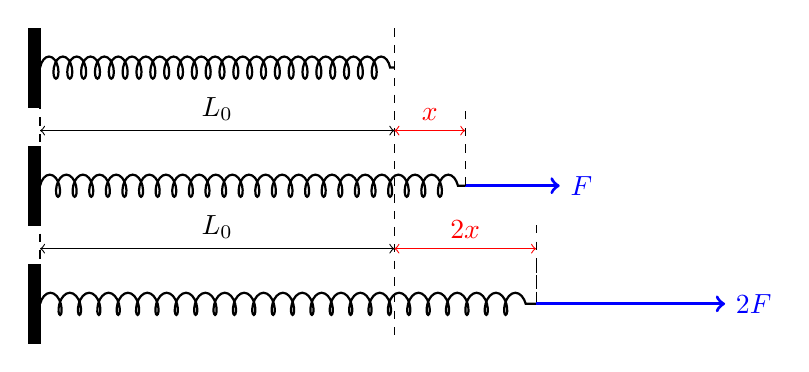
\begin{tikzpicture}[xscale=1.5]
	\draw[thick,decorate, decoration={coil,amplitude=4pt, segment length=5pt}] (0,0) -- (3,0);
	\draw[fill] (-0.1,-0.5) rectangle (0,0.5);
	\draw[dashed] (4.2,-2.5) -- (4.2,-3);
	\draw[thick,decorate, decoration={coil,amplitude=4pt, segment length=6pt}] (0,-1.5) -- (3.6,-1.5);
	\draw[fill] (-0.1,-2) rectangle (0,-1);
	\draw[very thick,blue,->] (3.6,-1.5) -- (4.4,-1.5) node[right]{$F$};
	\draw[thick,decorate, decoration={coil,amplitude=4pt, segment length=7pt}] (0,-3) -- (4.2,-3);
	\draw[fill] (-0.1,-3.5) rectangle (0,-2.5);
	\draw[very thick,blue,->] (4.2,-3) -- (5.8,-3) node[right]{$2F$};
	\draw[dashed] (0,0) -- (0,-3);
	\draw[dashed] (3,0.5) -- (3,-3.5);
	\draw[dashed] (3.6,-1.5) -- (3.6,-.5);
	\draw[<->] (0,-.8) -- (3,-.8) node[midway,above]{$L_0$};
	\draw[<->,red] (3,-.8) -- (3.6,-.8) node[midway,above]{$x$};
	\draw[dashed] (4.2,-2) -- (4.2,-3);
	\draw[<->] (0,-2.3) -- (3,-2.3) node[midway,above]{$L_0$};
	\draw[<->,red] (3,-2.3) -- (4.2,-2.3) node[midway,above]{$2x$};
	\end{tikzpicture}
\end{figure}

\cmt Hooke's law can be summarised by the equation: $\boxed{F=kx}$

\cmt the proportionality constant $k$ is called the \keypoint{spring constant}, or \keypoint{force constant}

larger $k$ means a greater force is required to extend the spring by same amount

a spring with a large $k$ is said to be \emph{stiff}

\cmt Hooke's law also holds if spring is being compressed

i.e., if a spring is pushed to have compression of $x$, we still have force applied $F=kx$

\cmt linear relationship between $F$ and $x$ is only true up to a certain range

the limit at which Hooke's law no longer holds is called the \keypoint{limit of proportionality}

\cmt if load is too large, spring might be overstretched and no longer exhibits elastic behaviour

the point beyond which spring cannot return to original length is called the \keypoint{elastic limit}
\footnote{The elastic limit of a spring and the limit of proportionality are two different but always confused concepts. These two limits are usually very close to one another, but they are conceptually different.}

\begin{figure}[ht]
	\centering
	\begin{tikzpicture}[yscale=0.96]
	\draw[<->] (9.6,0) node[below]{$x$} -- (0,0) -- (0,6.4) node[left]{$F$};
	\draw[thick] (0,0) -- (3,4) [out=53.13,in=185] to (9,6); \fill (3,4) circle(0.08); \fill (4.2,5.1) circle(0.08);
	\draw[<-] (1.8,2) -- ++(2.5,-0.8) node[note]{linear region for which \\ Hooke's law $F=kx$ holds};
	\draw[<-] (3.2,3.8) -- ++(1,-1) node[note]{limit of \\porportionality};
	\draw[<-] (3.9,5.2) -- ++(-1.5,.4) node[note]{elastic limit};
	\draw[<-] (6.4,5.5) -- ++(.8,-1.2) node[note]{non-linear region\\ where spring\\behaves plastically};
	\end{tikzpicture}
	\caption*{force-extension graph for a typical spring under load}
\end{figure}

\example{A spring has a natural length of 20.0 cm. When a mass of 250 g is suspended from the spring, the new length of the spring is 26.0 cm. Find the spring constant. }

\solc\begin{equation*}
	k = \frac{F}{x} = \frac{mg}{L-L_0} = \frac{0.250\times9.81}{(26.0-20.0)\times10^{-2}} \RA k \approx 40.9 \text{ N m}^{-1} \teoe
\end{equation*}

\example{A spring has a spring constant of $270 \text{ N m}^{-1}$. A mass of 1.2 kg is hung from the spring. When the mass is released from a position where the spring has an extension of 5.0 cm, what is the acceleration of the mass?}

\solc\begin{equation*}
	\fnet = F - mg = kx - mg = ma \RA a = \frac{kx-mg}{m} = \frac{270\times5.0\times10^{-2} - 1.2 \times 9.81}{1.2} \approx 1.44 \mpss \teoe
\end{equation*}

\subsubsection{elastic potential energy in a spring}\label{ch-spring-energy}

to stretch or compress a spring, work must be done

this becomes of \emph{elastic potential energy} stored in the spring \index{energy!elastic potential}


\begin{wrapfigure}{r}{0.36\textwidth}
	\vspace{0pt}
	\centering
		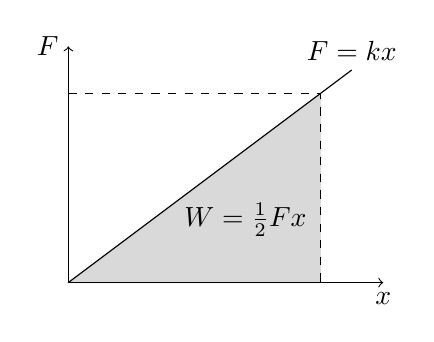
\begin{tikzpicture}[scale=1]
		\draw[gray!30,fill] (0,0) -- (3.2,0) -- (3.2,2.4) -- cycle;
		\draw[<->] (4,0) node[below]{$x$} -- (0,0) -- (0,3) node[left]{$F$};
		\draw (0,0) -- (3.6,2.7) node[above]{$F=kx$};
		\draw[dashed] (0,2.4) -- (3.2,2.4) -- (3.2,0);
		\node at (2.25,0.8) {$W=\frac{1}{2}Fx$};
		\end{tikzpicture}
	\vspace{-15pt}
\end{wrapfigure}

note that force in spring varies as spring is stretched

to find work in stretching a spring by $x$, we compute area under $F$-$x$ graph\footnote{Mathematically, we can also integrate over the total extension to find this work done $W=\int_0^x F \dd x = \int_0^x k x \dd x = \frac{1}{2}kx^2$, which of course gives the same result.}, which is a right-angled triangle

{
	\centering
	
	$ W = \frac{1}{2}Fx = \frac{1}{2}kx^2 $
	
}



so elastic potential energy stored in a spring is:

{
	\centering
	
	$ \boxed{E_p=\frac{1}{2}kx^2} $
	
}

\example{A steel spring has a spring constant of $20 \text{ N cm}^{-1}$. How much work is needed to stretch it from an extension of 3.0 cm to an extension of 5.0 cm?}

\sol work done needed equals the increase in elastic potential energy:
\begin{equation*}
	W = \Delta E_p = \frac{1}{2}kx_2^2 - \frac{1}{2}kx_1^2 = \frac{1}{2} \times 2000 \times (0.050^2 - 0.030^2) = 1.6 \text{ J} \teoe
\end{equation*}

\example{A trolley of 400 g can travel freely along a horizontal surface. It is pushed against a spring buffer. Suppose the spring is initially compressed by 5.0 cm under a 20 N force. When the trolley is released, it accelerates until it becomes detached. What is the trolley's final speed?}

\sol elastic potential energy in spring transforms into kinetic energy of trolley
\begin{equation*}
\frac{1}{2}Fx = \frac{1}{2}mv^2 \RA \frac{1}{2}\times20\times0.050 = \frac{1}{2}\times0.40\times v^2 \RA v\approx 1.58\mps \teoe
\end{equation*}

\example{The same spring is now set between two trolleys $A$ and $B$ of mass 400 g and 600 g. Initially the spring is again compressed by 5.0 cm under a force of 20 N. After both trolleys are released, what are their final speeds?}

\begin{figure}[ht]
	\centering
	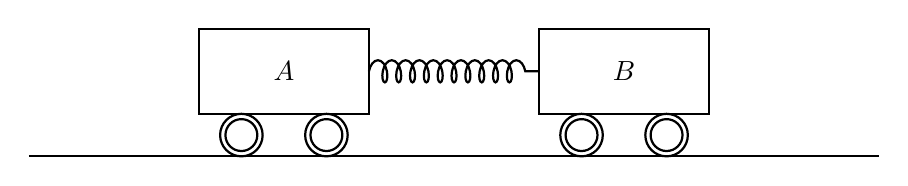
\begin{tikzpicture}[scale=1.35]
	\draw[thick,decorate, decoration={coil,amplitude=4pt, segment length=5pt}] (-.8,.4) -- (.8,.4);
	\draw[thick] (-2.4,0) rectangle (-.8,.8);
	\draw[thick] (.8,0) rectangle (2.4,.8);
	\foreach \c in {-2,-1.2,1.2,2}
	{  \draw[thick] (\c,-0.2) circle(0.2);
		\draw[thick] (\c,-0.2) circle(0.15);  }
	\draw[thick] (-4,-.4) -- (4,-.4);
	\node at (1.6,0.4) {$B$}; \node at (-1.6,0.4) {$A$};
	\end{tikzpicture}
\end{figure}

\sol elastic potential energy in spring transforms into kinetic energy of the two trolleys:
\begin{equation*}
\frac{1}{2}Fx=\frac{1}{2}m_Av_A^2 + \frac{1}{2}m_Bv_B^2 \RA 20\times0.050 = 0.40v_A^2 + 0.60v_B^2
\end{equation*}

total momentum for trolley $A$ and $B$ as a whole is conserved:
\begin{equation*}
m_Bv_B - m_Av_A = 0 \RA 0.40v_A = 0.60v_B
\end{equation*}

solving the simultaneous equations, we find: $v_A \approx 1.22\mps, v_B \approx 0.82 \mps$ \eoe

\subsubsection{spring combinations}

so far we have discussed the properties of a single spring

next we investigate how a set of springs respond to a given load

\subsubsection*{parallel springs}

\begin{wrapfigure}{r}{0.43\textwidth}
	\vspace{-15pt}
	\centering
	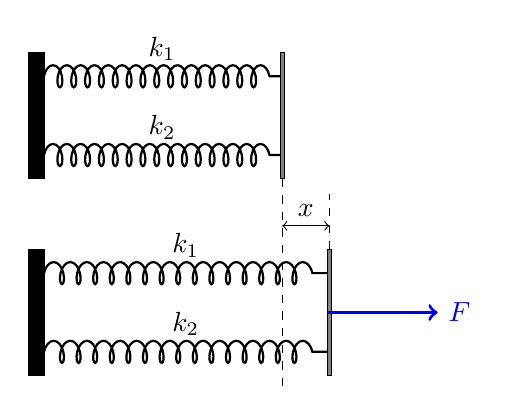
\begin{tikzpicture}[scale=1]
		\draw[thick,decorate, decoration={coil,amplitude=4pt, segment length=5pt}] (0,-0.5) -- (3,-0.5) node[midway,yshift=10pt]{$k_2$};
		\draw[thick,decorate, decoration={coil,amplitude=4pt, segment length=5pt}] (0,0.5) -- (3,0.5) node[midway,yshift=10pt]{$k_1$};
		\draw[fill] (-0.2,-0.8) rectangle (0,0.8);
		\draw[fill=black!50] (3,-0.8) rectangle (3.05,0.8);
		
		\draw[thick,decorate, decoration={coil,amplitude=4pt, segment length=6pt}] (0,-3) -- (3.6,-3) node[midway,yshift=10pt]{$k_2$};
		\draw[thick,decorate, decoration={coil,amplitude=4pt, segment length=6pt}] (0,-2) -- (3.6,-2) node[midway,yshift=10pt]{$k_1$};
		\draw[fill] (-0.2,-3.3) rectangle (0,-1.7);
		\draw[fill=black!50] (3.6,-3.3) rectangle (3.65,-1.7);
		\draw[very thick,blue,->] (3.6,-2.5) -- (5,-2.5) node[right]{$F$};
		\draw[dashed] (3.025,-0.8) -- (3.025,-3.5);
		\draw[dashed] (3.625,-1.7) -- (3.625,-1);
		\draw[<->] (3.025,-1.4) -- (3.625,-1.4) node[midway,above]{$x$};
	\end{tikzpicture}
%	\caption*{two springs in parallel}
	\vspace{-10pt}
\end{wrapfigure}

let's take two springs connected in parallel

when the combination is stretched under a load of $F$, extension in each spring should be the same:

{
	\centering
	
	$x_1=x_2=x$
	
}

the forces in each spring will in general be different, but sum of these must be equal to load: 

{
	\centering
	
	$ F=F_1+F_2 $
	
}


divide both sides by $x$, we have: $\frac{F}{x} = \frac{F_1}{x_1} + \frac{F_2}{x_2}$.

recall the Hooke's law, this becomes: $k=k_1+k_2$

generalize for $n$ springs in parallel connection, the combined spring constant is
\begin{equation*}
\boxed{k=k_1+k_2+\cdots+k_n}
\end{equation*}

\subsubsection*{series springs}

let's now take two springs in series

\begin{figure}[ht]
	\centering
	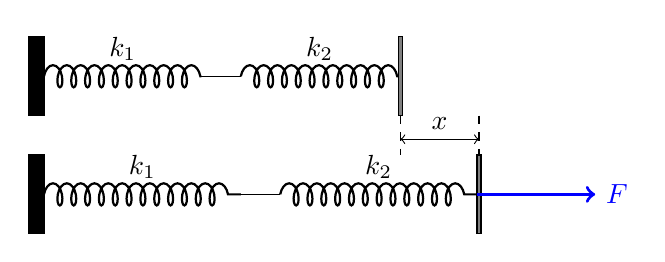
\begin{tikzpicture}[scale=1]
	\draw[thick,decorate, decoration={coil,amplitude=4pt, segment length=5pt}] (0,0) -- (2,0) node[midway,yshift=10pt]{$k_1$};
	\draw[thick,decorate, decoration={coil,amplitude=4pt, segment length=5pt}] (2.5,0) -- (4.5,0) node[midway,yshift=10pt]{$k_2$};
	\draw (2,0) -- (2.5,0);
	\draw[fill] (-0.2,-0.5) rectangle (0,0.5);
	\draw[fill=black!50] (4.5,-0.5) rectangle (4.55,0.5);
	
	\draw[thick,decorate, decoration={coil,amplitude=4pt, segment length=5pt}] (0,-1.5) -- (2.5,-1.5) node[midway,yshift=10pt]{$k_1$};
	\draw[thick,decorate, decoration={coil,amplitude=4pt, segment length=5pt}] (3,-1.5) -- (5.5,-1.5) node[midway,yshift=10pt]{$k_2$};
	\draw (2.5,-1.5) -- (3,-1.5);
	\draw[fill] (-0.2,-2) rectangle (0,-1);
	\draw[fill=black!50] (5.5,-2) rectangle (5.55,-1);
	\draw[very thick,blue,->] (5.5,-1.5) -- (7,-1.5) node[right]{$F$};
	\draw[dashed] (4.525,-0.5) -- (4.525,-1);
	\draw[dashed] (5.525,-0.5) -- (5.525,-1);
	\draw[<->] (4.525,-0.8) -- (5.525,-0.8) node[midway,above]{$x$};
	\end{tikzpicture}
%	\caption*{two springs in series}
\end{figure}


force in each spring is the same: $F_1=F_2=F$

but total extension is the sum of individual extensions: $x=x_1+x_2$.

divide by the same $F$, we have: $\frac{x}{F} = \frac{x_1}{F_1} + \frac{x_2}{F_2}$.

for combined spring constant, we find: $\frac{1}{k} = \frac{1}{k_1} + \frac{1}{k_2}$

for $n$ springs connected in series, the combined spring constant is therefore given by
\begin{equation*}
\boxed{\frac{1}{k} = \frac{1}{k_1} + \frac{1}{k_2} + \cdots \frac{1}{k_n}}
\end{equation*}

\subsubsection*{some brief remarks}

\cmt if we set up $n$ springs in parallel, we actually make it thicker

it then requires a stronger force to stretch it by the same extension

so we indeed see the combined spring constant is greater than that of any individuals

\cmt if we set up $n$ springs in series, we make it longer

instead of pulling one spring at a time, the same force now stretches $n$ springs simultaneously

this gives rise to a greater total extension

so the combined spring constant must be less than that of any individual

\example{(a) A spring with $k_1 = 20 \text{ N cm}^{-1}$ is connected in series with a second spring with $k_2 = 30 \text{ N cm}^{-1}$. When a force of 60 N is applied, what is the total extension of the combination? (b) The same two springs are now connected in parallel. When a force of 50 N is applied on the combination, what is the extension?}

\sol for series connection: $k = \left(\frac{1}{k_1} + \frac{1}{k_1}\right)^{-1} = \left( \frac{1}{20} + \frac{1}{30} \right)^{-1} = 12 \text{ N cm}^{-1} \RA x = \frac{F}{k} = \frac{60}{12} = 5.0 \text{ cm}$

\eqskip or sum up extension of each spring: $x = x_1 + x_2 = \frac{F}{k_1} + \frac{F}{k_2} = \frac{60}{20} + \frac{60}{30} = 5.0 \text{ cm}$

for parallel connection: $k = k_1 + k_2 = 20 + 30 = 50 \text{ N cm}^{-1} \RA x = \frac{F}{k} = \frac{50}{50} = 1.0 \text{ cm} $ \eoe

\begin{wrapfigure}{r}{0.25\textwidth}
	\vspace*{-5pt}
	\centering
	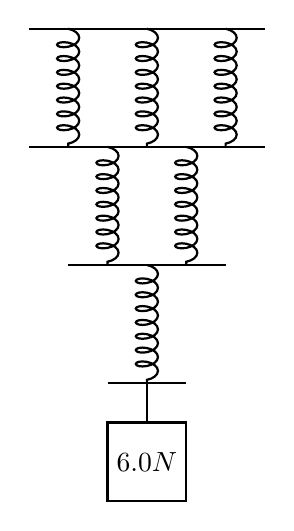
\begin{tikzpicture}
	\draw[thick] (-1.5,0) -- (1.5,0);
	\foreach \x in {-1,0,1}
	\draw[thick,decorate, decoration={coil,amplitude=4pt, segment length=5pt}] (\x,0) --++ (0,-1.5);
	\draw[thick] (-1.5,-1.5) -- (1.5,-1.5);
	\foreach \x in {-0.5,0.5}
	\draw[thick,decorate, decoration={coil,amplitude=4pt, segment length=5pt}] (\x,-1.5) --++ (0,-1.5);
	\draw[thick] (-1,-3) -- (1,-3);
	\draw[thick,decorate, decoration={coil,amplitude=4pt, segment length=5pt}] (0,-3) --++ (0,-1.5);
	\draw[thick] (-0.5,-4.5) -- (0.5,-4.5);
	\draw[thick] (0,-4.5) --++ (0,-0.5);
	\draw[thick] (-0.5,-6) rectangle (0.5,-5);
	\node at (0,-5.5) {$6.0 \text{ N}$};
	\end{tikzpicture}
	\vspace*{-16pt}
\end{wrapfigure}


\example{A set of identical springs are set up as shown. Each individual spring extends by 1.0 cm under a load of 1.0 N. Assume the limit of proportionality is not exceeded, what is the total extension for this combination when a load of 6.0 N is applied?}

\sol for a single spring: $k = 1.0 \text{ N cm}^{-1}$

combined spring constant: $k_\text{total} = \left( \frac{1}{3k} + \frac{1}{2k} + \frac{1}{k} \right)^{-1}$

{
	\centering
	
	\eqyskip $ k_\text{total} = \left(\frac{1}{3.0} + \frac{1}{2.0} + \frac{1}{1.0} \right)^{-1} = \frac{6}{11} \approx 0.545 \text{ N cm}^{-1}$
	
}

\eqyskip total extension: $x = \frac{F}{k_\text{total}} = \frac{6.0}{0.545} = 11 \text{ cm}$

alternatively, we can find and add extensions of each layer

in particular, the top layer withstands a force of 6.0 N shared by three springs, so each spring has a force of 2.0 N, extension is 2.0 cm

similarly, the other two layers extend by 3.0 cm and 6.0 cm respectively

hence, total extension: $x = 2.0 + 3.0 + 6.0 = 11 \text{ cm}$ \eoe




\subsection{stress, strain \& Young modulus}

from daily experience, it is easier to stretch a longer wire than a shorter one

same tensile force also produce greater effects on a thinner material than on a thicker one

so we need better quantities to describe the amount of deformation and the amount of action

to study a material's response to a tensile force, several new quantities are to be introduced

\subsubsection{stress \& strain}

\begin{ilight}
	\centering \keypoint{tensile strain}\index{strain} is defined as the ratio of the extension of a wire to its natural length: $\boxed{\epsilon = \frac{x}{L}}	$
\end{ilight}

\begin{ilight}
	\centering \keypoint{tensile stress}\index{stress} is defined as the force applied per unit cross-sectional area: $\boxed{\sigma = \frac{F}{A}}$ 
\end{ilight}

\cmt strain is the ratio of two lengths, so it is unit free

strain is usually expressed in terms of a percentage number

\cmt units of stress: $[\sigma] = \text{N m}^{-2} = \text{Pa}$ (pascal)

\cmt elastic behaviour of a wire is more or less like that of a spring

Hooke's law says $F \propto x$, it then follows that $\frac{F}{A} \propto \frac{x}{L}$, so $\sigma \propto \epsilon$

i.e., stress and strain should also be proportional to each other within certain limit

\example{A copper wire has a cross-sectional area of $1.5 \times 10^{-6} \text{ m}^2$. The breaking stress of the wire is $2.0 \times 10^8 \text{ Pa}$. Find the breaking force.}

\solc\begin{equation*}
\sigma = \frac{F}{A} \RA F = \sigma A = 2.0 \times 10^8 \times 1.5 \times 10^{-6} = 3.0 \times 10^2 \text{ N} \teoe
\end{equation*}

\subsubsection{Young modulus}

\begin{ilight}
	\centering ratio of stress to strain of a material is called the \keypoint{Young modulus}\index{Young modulus}: $ \boxed{E = \frac{\sigma}{\epsilon}}$
\end{ilight}


\cmt unit of measurement: $[E] = \text{Pa}$ (pascal)

\cmt Young modulus is a property of the material

for the same material, Young modulus is a constant, no matter in what shape it takes

i.e., it does not depend on the length or the cross section of the object

\cmt typical value of Young's modulus for metals: $E_\text{metal} \sim 10^{11} \text{ Pa}$

\cmt Young modulus is a measure of the stiffness of a material

to produce same strain, greater stress is required for a material with greater Young modulus

\cmt Young modulus $E$ is related to the force constant $k$

from $E = \frac{\sigma}{\epsilon} = \frac{\sfrac{F}{A}}{\sfrac{x}{L}} = \frac{FL}{xA}$, we rearrange to get: $F = \frac{EA}{L}x$

compare with Hooke's law, we can identify the force constant to be given by: $k = \frac{EA}{L} $

\titem $E \up \ra k \up$, stiffer material makes stiffer springs

\titem $A \up \ra k \up$, more difficult to stretch a thick spring (think about parallel springs)

\titem $L \up \ra k \down$, easier to stretch a long spring (think about series springs)

\example{A 200 N tensile force is applied on a steel wire of 1.5 m, the wire extends by 5.0 mm. The diameter of the cross section is 0.60 mm. What is the Young modulus of the steel wire?}

\solc\begin{equation*}
	E = \frac{\sigma}{\epsilon} = \frac{\sfrac{F}{A}}{\sfrac{x}{L}} = \frac{FL}{Ax} = \frac{200 \times 1.5}{\pi \times (0.30\times10^{-3})^2 \times 5.0 \times 10^{-3}} \RA E \approx 2.1 \times 10^{11} \text{ Pa} \teoe
\end{equation*}

\example{A copper wire of length 2.0 m is under a stress of $7.8 \times 10^7 \text{ Pa}$. Given that the Young modulus of copper is $1.2 \times 10^{11} \text{ Pa}$, what is (a) the strain of the wire, (b) the extension of the wire?}

\sol strain: $\epsilon = \frac{\sigma}{E} = \frac{7.8 \times 10^7}{1.2 \times 10^{11}} \RA \epsilon = 6.5 \times 10^{-4} = 0.065 \%$

extension: $x = \epsilon L = 6.5 \times 10^{-4} \times 2.0 \RA x = 1.3 \times 10^{-3} \text{ m}$ \eoe

\example{Several blocks of steel are used to support a bridge. Each block has a height of 30 cm and a cross section of 15 cm $\times$ 15 cm. The steel block is designed to compress 2.0 mm when the maximum load is applied. Given that the Young modulus of steel is $2.1 \times 10^{11} \text{ Pa}$, what is the maximum load that can be supported by one block?}

\solc\begin{equation*}
	E = \frac{FL}{Ax} \RA F = \frac{EAx}{L} = \frac{2.1\times10^{11} \times (0.15\times0.15) \times2.0\times10^{-3}}{0.30} \RA F \approx 3.15 \times 10^7 \text{ N} \teoe
\end{equation*}


\example{Two metal wires $A$ and $B$ are of the same length and they extend by the same amount under the same load. Given that Young modulus of wire $A$ is twice of $B$, what is the ratio of their diameters?}

\solc\begin{equation*}
	E = \frac{FL}{Ax} \RA A = \frac{1}{4}\pi d^2 = \frac{FL}{Ex} \RA d^2 \propto \frac{1}{E} \RA \frac{d_A}{d_B} = \sqrt{\frac{E_B}{{E_A}}} = \frac{1}{\sqrt{2}} \teoe
\end{equation*}


\example{A full-size crane is ten times greater than a model crane in all linear dimensions. If they are made of the same materials, what is the ratio of the cable's extension?}

\sol same material means same density $\rho$ and same Young's modulus $E$, so:
\begin{equation*}
E = \frac{FL}{Ax} \RA x = \frac{FL}{AE} = \frac{mgL}{\pi r^2 E} = \frac{\rho V g L}{\pi r^2 E} \RA x \propto \frac{VL}{r^2} \propto \frac{l^3 l}{l^2} \propto l^2 \RA \frac{x_\text{full}}{x_\text{model}} = 10^2 = 100 \teoe
\end{equation*}


\subsubsection{measurement of Young modulus}\label{ch-measure-E}

to measure Young's modulus of a metal wire, experimental setup can be laid out as shown


\begin{figure}[ht]
	\centering
	\begin{tikzpicture}
	\draw[thick] (0,-0.1) -- (0,1.5);
	\foreach \y in {0.2,0.4,...,1.4} \draw[thick] (0,\y) --++ (-0.2,-0.2);
	\draw[thick] (-0.3,-0.1) -- (11.1,-0.1) -- (11.1,-3.5);
	\draw[thick,fill=white] (11.2,0) circle (0.78);
	\draw[very thick,gray] (0,0.8) -- (11.2,0.8) arc (90:0:0.8) -- (12,-1.5);
	\draw[thick,fill] (11.25,0) --++ (0.05,-0.05) --++ (-.9,-.9) --++ (-0.05,0.05) -- cycle; 
	\draw (5,0.9) --++ (1,1) node[above]{metal wire};
	\draw[Green,fill=blue] (7.9,0.9) -- (8.1,0.9) -- (8,0.6) -- cycle;
	\draw (8,1) --++ (1,1) node[above]{marker};
	\draw (11.4,0.6) --++ (1,1) node[above]{pulley};
	\draw[thick,fill=white] (7.5,0) rectangle (9,-0.2);
	\draw[thick,fill=white] (8,0.05) circle(0.16);
	\draw (8,-0.3) --++ (-1,-1) node[below,twoline]{travelling\\microscope};
	\foreach \y in {-2.9,-2.25,-1.6} {
		\draw[thick] (11.84,\y-0.04) arc (180:0:0.16) [out=-90, in=90] to (12, \y-0.3);
		\draw[thick,fill=white] (11.6,\y-0.6) rectangle (12.4,\y-0.3);
	}
	\draw (12.5,-2) --++ (.8,.8) node[above]{masses};
	\end{tikzpicture}
\end{figure}

\cmt method of data collection

\titem original length $L$ (up to the marker) of the wire is measured with \emph{metre rule}

\titem diameter $d$ of the wire is measured with \emph{micrometer}, then cross-sectional area is: $A = \frac{1}{4}\pi d^2$

\titem record mass $m$ attached to the wire, then force applied is $F=mg$

\titem extension $x$ of the wire is taken to be distance moved out by the marker

\phantom{\titem}this can be measured with a \emph{travelling microscope}\footnote{A travelling microscope is basically a microscope that can move back and forth along a rail. The position of the microscope can be varied by turning a screw. This position can be read off a vernier scale. So in short, a travelling microscope can be used to measure the change in length with a very high resolution (typically to a precision of 0.01mm or 0.02 mm).} or a \emph{vernier calliper}

\cmt analysis of data

stress can be calculated by $\sigma = \frac{F}{A}$, and strain can be calculated by $\epsilon = \frac{x}{L}$

a graph of stress against strain can be plotted, a best fit curve can be drawn

gradient of the straight-line section gives Young modulus




\subsubsection{stress-strain curves}

stress-strain curve for a material can be obtained using the methods in \S\ref{ch-measure-E}

in AS-Level, you are only supposed to know the behaviour of a metal under stress

\begin{figure}[ht]
	\centering
	\begin{tikzpicture}[scale=0.85]
	\draw[<->] (9.6,0) node[below]{strain} -- (0,0) -- (0,6.4) node[left]{stress};
	\draw[thick] (0,0) -- (3,4) [out=53.13,in=185] to (9,6); \fill (3,4) circle(0.08);
	\fill (4.2,5.1) circle(0.08);
	\fill (9,6) circle(0.08);
	\draw[<-] (1.8,2) -- ++(2.3,-0.9) node[note]{linear\\region};
	\draw[<-] (3.2,3.8) -- ++(1,-1) node[note]{$L_P$: limit of \\porportionality};
	\draw[<-] (3.9,5.2) -- ++(-1.5,.4) node[note]{$L_E$: limit\\ of elasticity};
	\draw[<-] (6.5,5.6) -- ++(.2,-1.5) node[note]{plastic flow};
	\draw[<-] (9,5.8) -- ++(.1,-1.2) node[note]{breaking\\point};
	\end{tikzpicture}
	\caption*{stress-strain graph for a typical metal}
\end{figure}

\cmt up to limit of proportionality $L_E$, stress is proportional to strain

Young modulus can be given by the gradient of the curve before $L_P$

\cmt consider the product of stress and strain: $\sigma \cdot \epsilon \sim \frac{F}{A} \frac{x}{L} \sim \frac{Fx}{AL} \sim \frac{W}{V}$

so area under stress-strain curve gives the work done per unit volume to stretch the wire

\cmt up to limit of elasticity $L_E$, metal wire can return to original length when it relaxes

\begin{wrapfigure}{r}{0.40\textwidth}
	\vspace*{-15pt}
	\centering
	\begin{tikzpicture}[scale=0.62]
	\draw[fill=yellow!30] (0,0) -- (3,4) [out=53.13,in=190] to (7,5.7)  -- (2.725,0) -- cycle;
	\draw[fill=green!30] (7,5.7)  -- (2.725,0) -- (7,0) -- cycle;
	\draw[<->] (8,0) node[below]{strain} -- (0,0) -- (0,6.4) node[above]{stress};
	\draw[thick,blue,postaction={decorate},decoration={markings,mark=at position 0.45 with {\arrow{>}}}] (0,0) -- (3,4) [out=53.13,in=190] to (7,5.7);
	\draw[thick,blue,postaction={decorate},decoration={markings,mark=at position 0.6 with {\arrow{>}}}] (7,5.7) -- (2.725,0);
	\draw[thick] (7,5.7) [out=10,in=185] to (8,5.85);
	\fill (4.0,4.92) circle(0.08) node[above left] {$L_E$};
	\node[blue,rotate=53.13, above] at (2.4,3.2) {loading};
	\node[blue,rotate=53.13, below] at (4.6,2.5) {unloading};
	\node at (3.5,2.7) {{\Large $X$}};
	\node at (6,2) {{\Large $Y$}};
	\end{tikzpicture}
	\vspace*{-16pt}
\end{wrapfigure}

\cmt if a wire is stretched beyond the elastic limit, it follows a different path when force is removed

recall area under stress-strain graph relates to energy

work to stretch wire is given by $X+Y$

energy goes out when wire contracts is $Y$

the difference $X$ gives energy loss during one cycle

this energy difference becomes heat produced in wire








\ifthenelse{\includequestions=1}{
	
\subsection{end-of-chapter questions}


\subsubsection*{springs \& Hooke's law}

\question{A spring has a force constant of $500 \text{ N m}^{-1}$. The spring has a stretch length of 30 cm when a 40 N weight is hung from it. Find the natural length of the spring.}

\question{Two springs, one with spring constant $k_1 = 8.0 \text{ N cm}^{-1}$ and the other with $k_2 = 12 \text{ N cm}^{-1}$. (a) When they are connected in parallel, what is the total extension when the combination supports a load of 60 N? (b) If they are connected in series, what is the total extension when they support the same load?}

\question{A weight of 100 N is placed on top of a spring. The spring is compressed by 2.0 cm. Assume the spring obeys Hooke's law, how much strain energy is stored in the spring?}

\question{A spring with a force constant $800 \text{ N m}^{-1}$ is supported and stands vertically. A ball of mass 60 g falls vertically onto it. The ball has a speed of $3.0\mps$ as it makes contact with the spring. Assume no energy loss, what is the maximum compression of the spring?}

\question{A trolley of mass 160 g is placed on a frictionless track. The trolly pushed against a spring buffer of a force constant $90 \text{ N m}^{-1}$. The spring buffer is compressed by 7.0 cm. The trolley is then released from rest. (a) What is the initial acceleration of the trolley? (b) Assume no loss of energy, what is the final speed of the trolley along the track?}

\question{
	Spring $A$ is stiffer than spring $B$, i.e., $k_A>k_B$. On which spring is more elastic potential energy stored if they are stretched by (a) the same extension, (b) the same force?
}

\begin{wrapfigure}{r}{0.47\textwidth}
	\vspace*{-5pt}
	\centering
	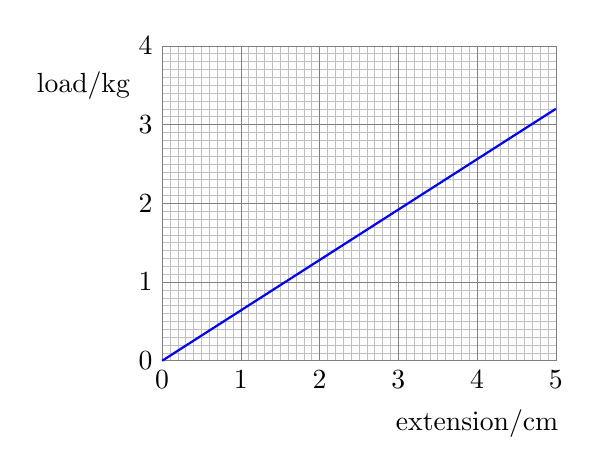
\begin{tikzpicture}
	\draw[help lines, gray!50, very thin, step=0.1] (0,0) grid (5,4);
	\draw[help lines, step=1] (0,0) grid (5,4);
	\foreach \y in {0,1,2,3, 4} \node[left] at (0,\y) {$\y$};
	\foreach \x in {0,1,2,3,4,5} \node[below] at (\x,0) {$\x$};
	\node at (-1,3.5) {load/kg};
	\node at (4,-0.8) {extension/cm};
	\draw[thick,blue] (0,0) -- (5,3.2);
	\end{tikzpicture}
	\vspace*{-25pt}
\end{wrapfigure}

\question{A load is attached to the lower end of a spring. The extension of the spring is measured when the load increases. The variation with extension of the load is shown. (a) Suggest whether the spring obeys Hooke's law. (b) Find the spring constant. (c) How much elastic potential energy is stored in the spring when the extension is 5.0 cm? (d) How much work is done to increase the extension from 2.0 cm to 4.0 cm?}


\question{
	Suppose you have a spring, a ruler, a mass hanger and a set of masses. Suggest how the apparatus may be used to determine the load on the spring at (a) the limit of elasticity, (b) the limit of proportionality?
}


\subsubsection*{stress, strain, \& Young modulus}

\question{A cable of diameter 1.5 mm is under a tension of 200 N. Find the stress in this cable.}

\question{Estimate the stress in your neck when it supports your head in a vertical position.}

\question{A metal wire of natural length 1.8 m and diameter 0.70 mm is fixed to the ceiling at one end. When a mass of 6.5 kg is hung from the lower end, the wire extends by 2.7 mm. (a) Find the strain of the wire. (b) Find the Young modulus of the metal.}

\question{A wire has a diameter of 0.50 mm with a Young modulus of 0.18 TPa. The length of the wire is increased by 0.20\% by a force $F$. (a) Find the stress in the wire. (b) Find the force $F$.}


\question{Two metal wires $A$ and $B$ are made of different materials. The diameter of wire $A$ is twice that of wire $B$, and the Young modulus of wire $A$ is three times that of wire $B$. If the wires are extended by the same strain, what is the ratio of the tension in wire $A$ to tension in wire $B$?}



\question{Two rods $A$ and $B$ of the same diameter are joined end to end and hug vertically. Rod $B$ is twice as long as rod $A$ but has half the Young modulus. When a mass is hung from the combination, what is the ratio of the extension of rod $A$ to the extension of rod $B$?}

\question{Bones of different animals have very similar compositions. Suggest why heavier animals appear to have thicker bones?}


\begin{wrapfigure}{r}{0.45\textwidth}
	\vspace*{5pt}
	\centering
	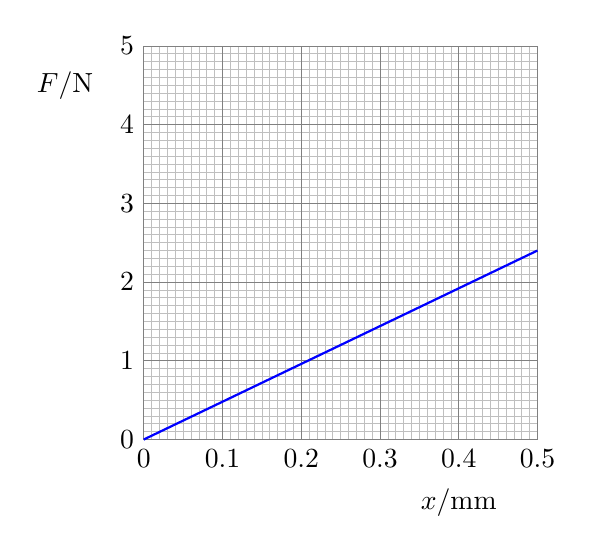
\begin{tikzpicture}
	\draw[help lines, gray!50, very thin, step=0.1] (0,0) grid (5,5);
	\draw[help lines, step=1] (0,0) grid (5,5);
	\foreach \y in {0,1,2,3,4,5} \node[left] at (0,\y) {$\y$};
	\foreach \x in {0,0.1,0.2,0.3,0.4,0.5} \node[below] at (10*\x,0) {$\x$};
	\node at (-1,4.5) {$F$/N};
	\node at (4,-0.8) {$x$/mm};
	\draw[thick,blue] (0,0) -- (5,2.4);
	\end{tikzpicture}
	\vspace*{-25pt}
\end{wrapfigure}

\question{A load $F$ is suspended from a copper wire. The graph shows the load-extension relation. (a) State two quantities other than $F$ and $x$ that are required to determine the Young modulus of copper. (b) Suggest how the two quantities may be measured. (c) Use the graph to find the energy stored in the wire when a load of 2.0 N is applied. (d) Given that steel has about twice the Young modulus as copper, sketch the variation with $x$ of $F$ for a steel wire that has the same dimensions as the copper wire.}

\begin{wrapfigure}{r}{0.40\textwidth}
	\vspace*{-10pt}
	\centering
	\begin{tikzpicture}[scale=0.54]
	\draw[<->] (6.4,0) node[below]{strain} -- (0,0) -- (0,6.4) node[left]{stress};
	\draw[thick,blue,postaction={decorate},decoration={markings,mark=at position 0.5 with {\arrow{>}}}] (0,0) [out=60,in=210] to (3,4) [out=30,in=225] to (6,6);
	\draw[thick,blue,postaction={decorate},decoration={markings,mark=at position 0.5 with {\arrow{>}}}] (6,6) [out=240,in=30] to (3,3) [out=210,in=50] to (0,0);
	\end{tikzpicture}
	\vspace*{-16pt}
\end{wrapfigure}

\question{
	In an experiment, a speciman of a rubber compound is being stretched and relaxed. The stress-strain curve is plotted. (a) State and explain whether this rubber compound behaves elastically. (b) The tyres on a vehicle are made of this rubber compound. Explain why the tyres become warm as the car travels on a road.
}

}{}